\documentclass[aspectratio=169,11pt]{beamer}

\usetheme{AnnArbor}
\usepackage{fontspec}
\usepackage{amsmath,amssymb,booktabs,array,multicol}
\usepackage{listings}
\usepackage{xcolor}
\usepackage{graphicx}
\usepackage{hyperref}
\usepackage{ragged2e}

\setmainfont{DejaVu Serif}
\setsansfont{DejaVu Sans}
\setmonofont{Noto Sans Mono}

\definecolor{CodeBg}{RGB}{248,248,248}
\definecolor{TitleBlue}{RGB}{38,79,129}
\definecolor{AccentGreen}{RGB}{35,125,93}
\definecolor{SoftGray}{RGB}{80,80,80}
\definecolor{QuizOrange}{RGB}{180,95,30}

\setbeamercolor{title}{fg=TitleBlue}
\setbeamercolor{frametitle}{fg=TitleBlue}
\setbeamercolor{structure}{fg=AccentGreen}
\setbeamercolor{block title}{fg=white,bg=TitleBlue}
\setbeamercolor{block body}{bg=blue!3}
\setbeamercolor{alertblock title}{fg=white,bg=QuizOrange}
\setbeamercolor{alertblock body}{bg=orange!6}
\setbeamertemplate{navigation symbols}{}
\setbeamertemplate{footline}[frame number]
\setbeamertemplate{itemize item}{\raise0.15ex\hbox{\tiny$\blacktriangleright$}}
\setbeamertemplate{itemize subitem}{\raise0.15ex\hbox{\tiny$\bullet$}}

\lstdefinestyle{py}{
  language=Python,
  basicstyle=\ttfamily\scriptsize,
  backgroundcolor=\color{CodeBg},
  frame=single,
  framerule=0.2pt,
  rulecolor=\color{gray!35},
  breaklines=true,
  showstringspaces=false,
  keywordstyle=\color{TitleBlue}\bfseries,
  commentstyle=\color{SoftGray}\itshape,
  stringstyle=\color{AccentGreen},
  upquote=true
}

\newcommand{\key}[1]{\textbf{\textcolor{AccentGreen}{#1}}}
\newcommand{\cmd}[1]{\texttt{\detokenize{#1}}}

\title[Truy xuất \& Lưu trữ Dữ liệu]{Truy xuất và Lưu trữ Dữ liệu với Python}
\subtitle{Tập tin phẳng (CSV), Đa định dạng (Excel, JSON, HTML, PDF), SQLite \& MongoDB}
\author{TS. Vũ Đức Minh}
\institute{Khoa Khoa học Dữ liệu \& Trí tuệ Nhân tạo -- Đại học Kinh tế Quốc dân (NEU)}
\date{Tháng 9, 2026}

\begin{document}

\begin{frame}
  \titlepage
\end{frame}

\begin{frame}{Mục tiêu bài học (CLO 5.4)}
\small
Sau khi hoàn thành bài học này, sinh viên có khả năng:
\begin{itemize}
  \item \key{Đọc \& ghi CSV:} Nắm vững \cmd{np.loadtxt}, \cmd{np.genfromtxt} và các tham số nâng cao của \cmd{pd.read_csv()} (\cmd{chunksize}, \cmd{encoding}, \cmd{parse_dates}).
  \item \key{Đa dạng định dạng tệp:} Làm việc với Excel đa trang tính (\cmd{openpyxl}), làm phẳng JSON lồng nhau (\cmd{json_normalize}), bóc tách bảng HTML và trích xuất PDF.
  \item \key{Cơ sở dữ liệu quan hệ:} Kết nối SQLite qua \cmd{sqlite3} \& \cmd{SQLAlchemy}, thực thi truy vấn SQL và chuyển đổi hai chiều với Pandas (\cmd{read_sql_query}, \cmd{to_sql}).
  \item \key{Cơ sở dữ liệu NoSQL:} Kết nối MongoDB qua \cmd{pymongo}, thực hiện thao tác CRUD, chuẩn hóa BSON \cmd{ObjectId} sang DataFrame.
  \item \key{End-to-End Pipeline:} Thiết kế quy trình thu thập dữ liệu đa nguồn phục vụ báo cáo kinh doanh.
\end{itemize}
\end{frame}

\begin{frame}{Tổng quan Hệ sinh thái Truy xuất \& Lưu trữ Dữ liệu}
\centering
\IfFileExists{images/data-access-storage-overview.png}{
  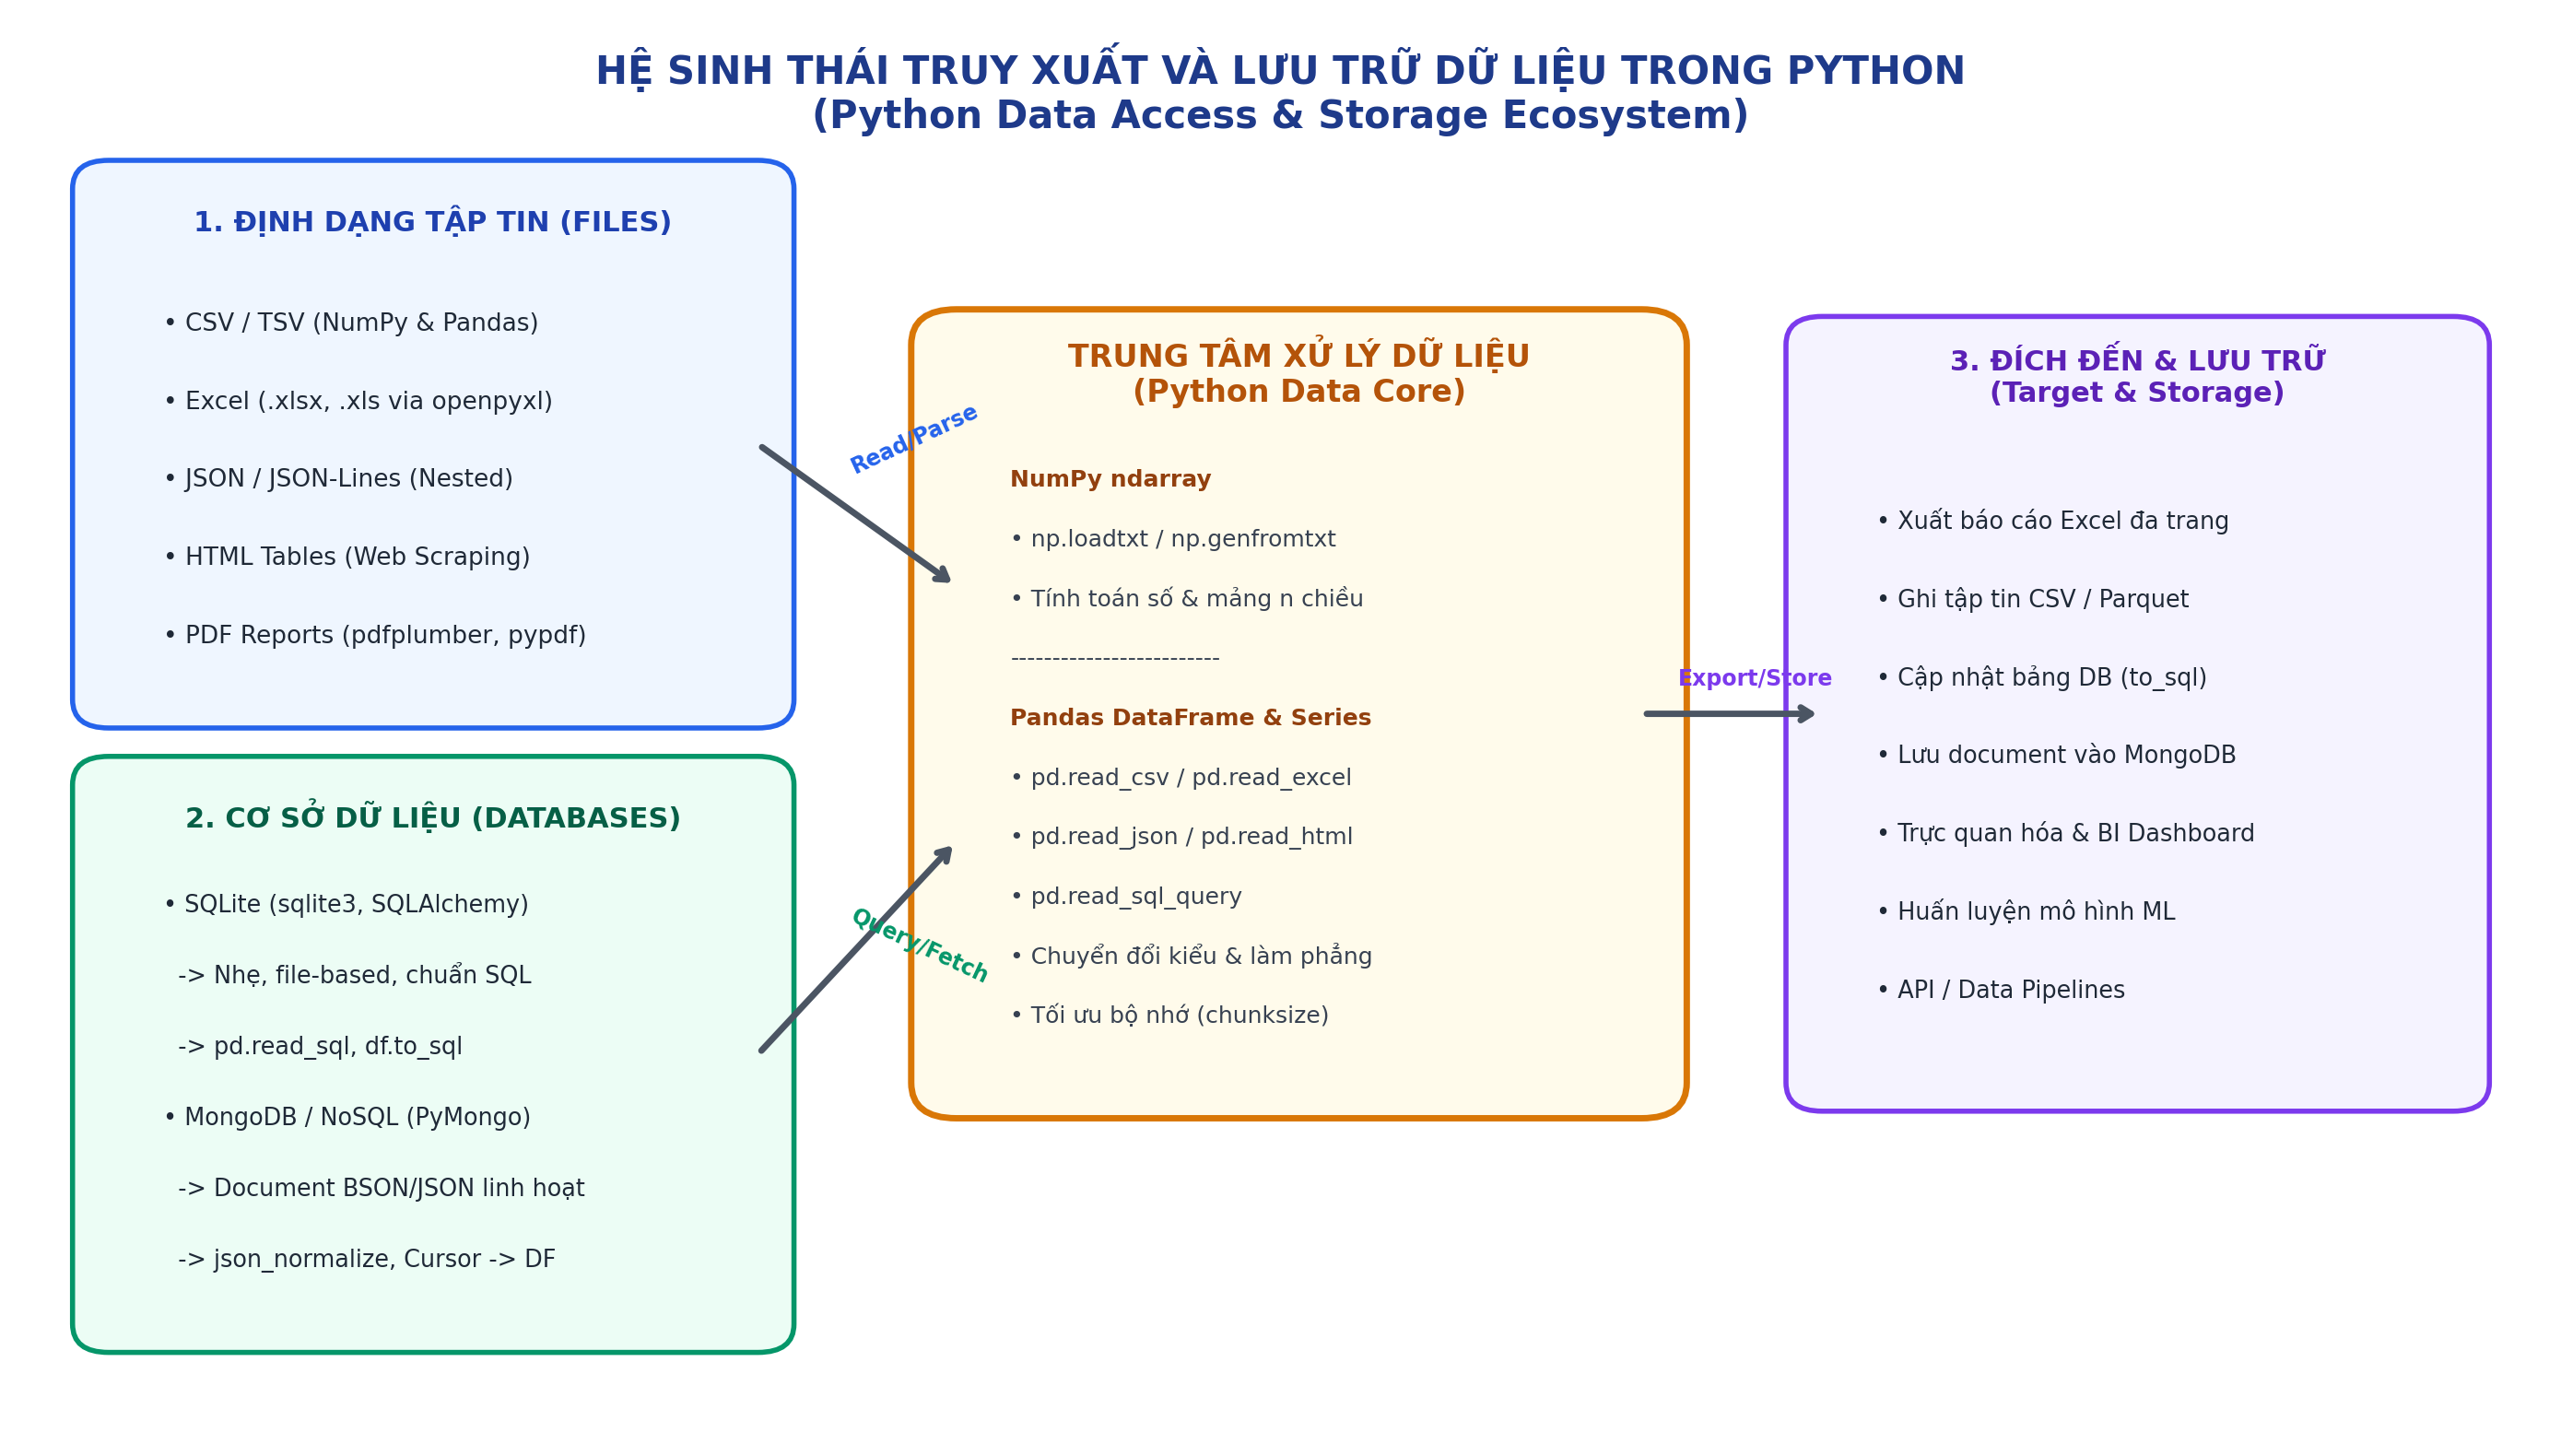
\includegraphics[width=0.92\linewidth]{images/data-access-storage-overview.png}
}{
  \begin{block}{Hệ sinh thái I/O}
  Files (CSV/Excel/JSON) \& Databases (SQLite/Mongo) $\rightarrow$ Pandas Core $\rightarrow$ Output Analytics
  \end{block}
}
\end{frame}

\begin{frame}[fragile]{Đọc dữ liệu CSV bằng NumPy}
\small
NumPy cung cấp hai hàm chính để làm việc với mảng số từ tệp văn bản:
\begin{columns}[T]
\column{0.48\linewidth}
\begin{block}{\cmd{np.loadtxt()}}
Dành cho dữ liệu số thuần túy, không có giá trị khuyết.
\begin{lstlisting}[style=py]
import numpy as np
# Doc ma tran so thuan tuy
arr = np.loadtxt("matrix.csv", 
                 delimiter=",", 
                 skiprows=1)
print(arr.shape)
\end{lstlisting}
\end{block}
\column{0.48\linewidth}
\begin{block}{\cmd{np.genfromtxt()}}
Xử lý được giá trị khuyết và kiểu dữ liệu hỗn hợp.
\begin{lstlisting}[style=py]
# Thay the gia tri thieu bang 0.0
arr_gen = np.genfromtxt(
    "numeric_sample.csv",
    delimiter=",",
    skip_header=1,
    filling_values=0.0
)
\end{lstlisting}
\end{block}
\end{columns}
\vspace{0.5em}
Xuất mảng ra CSV: \texttt{np.savetxt("out.csv", arr, delimiter=",", fmt="\%0.2f")}.
\end{frame}

\begin{frame}[fragile]{Các tham số trọng yếu của Pandas \cmd{read_csv()}}
\small
\begin{lstlisting}[style=py]
import pandas as pd

df = pd.read_csv(
    "data/customers.csv",
    sep=",",                         # Ky tu phan cach cot (mac dinh la ',')
    index_col="customer_id",         # Cot lam chi muc Index
    usecols=["customer_id", "full_name", "signup_date", "total_spent"], # Tiet kiem RAM
    dtype={"customer_id": str},      # Ep kieu ro rang tranh sai lech
    parse_dates=["signup_date"],     # Chuyen doi chuoi thanh kieu datetime
    na_values=["NA", "null", "-"],   # Cac ky tu quy uoc gia tri khuyet
    encoding="utf-8"                 # Ho tro tieng Viet chuan
)
\end{lstlisting}
\vspace{-0.3em}
\begin{alertblock}{Mẹo xuất CSV tiếng Việt mở trên Excel}
Dùng \cmd{df.to_csv("clean.csv", index=False, encoding="utf-8-sig")}. Cờ \cmd{utf-8-sig} bổ sung Byte Order Mark (BOM) giúp Excel tự nhận diện đúng tiếng Việt có dấu.
\end{alertblock}
\end{frame}

\begin{frame}[fragile]{Xử lý tệp CSV dung lượng lớn với \cmd{chunksize}}
\small
Khi tệp CSV vượt quá dung lượng bộ nhớ RAM, nạp toàn bộ sẽ gây lỗi \key{MemoryError}. Kỹ thuật \key{Chunking} giải quyết triệt để:

\begin{lstlisting}[style=py]
import pandas as pd

# Khoi tao bo lap streaming doc tung khoi 100,000 dong
chunk_iter = pd.read_csv("large_transactions.csv", chunksize=100000,
                         usecols=["store_id", "revenue"])

store_totals = {}
for i, chunk in enumerate(chunk_iter):
    # Xu ly tung khoi doc lap trong bo nho
    grouped = chunk.groupby("store_id")["revenue"].sum()
    for sid, rev in grouped.items():
        store_totals[sid] = store_totals.get(sid, 0) + rev
    print(f"-> Hoan tat xu ly chunk #{i+1}")

print("Tong doanh thu:", store_totals)
\end{lstlisting}
\end{frame}

\begin{frame}[fragile]{Làm việc với bảng tính Excel (\cmd{openpyxl})}
\small
\begin{columns}[T]
\column{0.48\linewidth}
\begin{block}{Đọc nhiều trang tính (Sheets)}
\begin{lstlisting}[style=py]
# Doc 1 sheet cu the
df = pd.read_excel("products.xlsx", 
                   sheet_name="Products", 
                   engine="openpyxl")

# Doc TAT CA cac sheet (tra ve dict)
all_sheets = pd.read_excel(
    "products.xlsx", 
    sheet_name=None, 
    engine="openpyxl"
)
\end{lstlisting}
\end{block}
\column{0.48\linewidth}
\begin{block}{Ghi nhiều Sheet vào 1 file}
\begin{lstlisting}[style=py]
# Ghi multi-sheet bang ExcelWriter
with pd.ExcelWriter("report.xlsx", 
                    engine="openpyxl") as w:
    df_prod.to_excel(w, 
                     sheet_name="Products", 
                     index=False)
    df_kpi.to_excel(w, 
                    sheet_name="Summary_KPI", 
                    index=False)
\end{lstlisting}
\end{block}
\end{columns}
\end{frame}

\begin{frame}[fragile]{Làm phẳng dữ liệu JSON phân cấp (\cmd{json_normalize})}
\small
Dữ liệu JSON từ Web APIs thường có cấu trúc lồng nhau phức tạp (\key{Nested Objects \& Arrays}).

\begin{lstlisting}[style=py]
import json, pandas as pd

with open("ecommerce_transactions.json", "r", encoding="utf-8") as f:
    orders = json.load(f)

# Lam phang mang 'items' dong thoi mang theo cac truong metadata cap cha
df_flat = pd.json_normalize(
    orders,
    record_path=["items"],                  # Phan tach tung dong theo tung item
    meta=["order_id", "order_date",         # Thuoc tinh goc cua order
          ["customer", "customer_id"],      # Truong con long nhau cap 2
          ["customer", "name"], 
          ["customer", "city"]]
)
print(df_flat.head(3))
\end{lstlisting}
\end{frame}

\begin{frame}[fragile]{Bóc tách Bảng từ Web HTML \& Báo cáo PDF}
\small
\begin{columns}[T]
\column{0.48\linewidth}
\begin{block}{Web Scraping bảng với \cmd{read_html}}
\begin{lstlisting}[style=py]
# Quet tat ca the <table> tu URL/file
tables = pd.read_html(
    "financial_quotes.html", 
    match="VN-Index" # Loc theo tu khoa
)
df_stocks = tables[0]
print(df_stocks.head())
\end{lstlisting}
\end{block}
\column{0.48\linewidth}
\begin{block}{Trích xuất bảng PDF (\cmd{pdfplumber})}
\begin{lstlisting}[style=py]
import pdfplumber

with pdfplumber.open("invoice.pdf") as pdf:
    for page in pdf.pages:
        tables = page.extract_tables()
        for t in tables:
            df = pd.DataFrame(t[1:], 
                              columns=t[0])
            print(df)
\end{lstlisting}
\end{block}
\end{columns}
\end{frame}

\begin{frame}{Mô hình Quan hệ (SQLite) vs Hướng tài liệu (MongoDB)}
\centering
\IfFileExists{images/relational-vs-nosql.png}{
  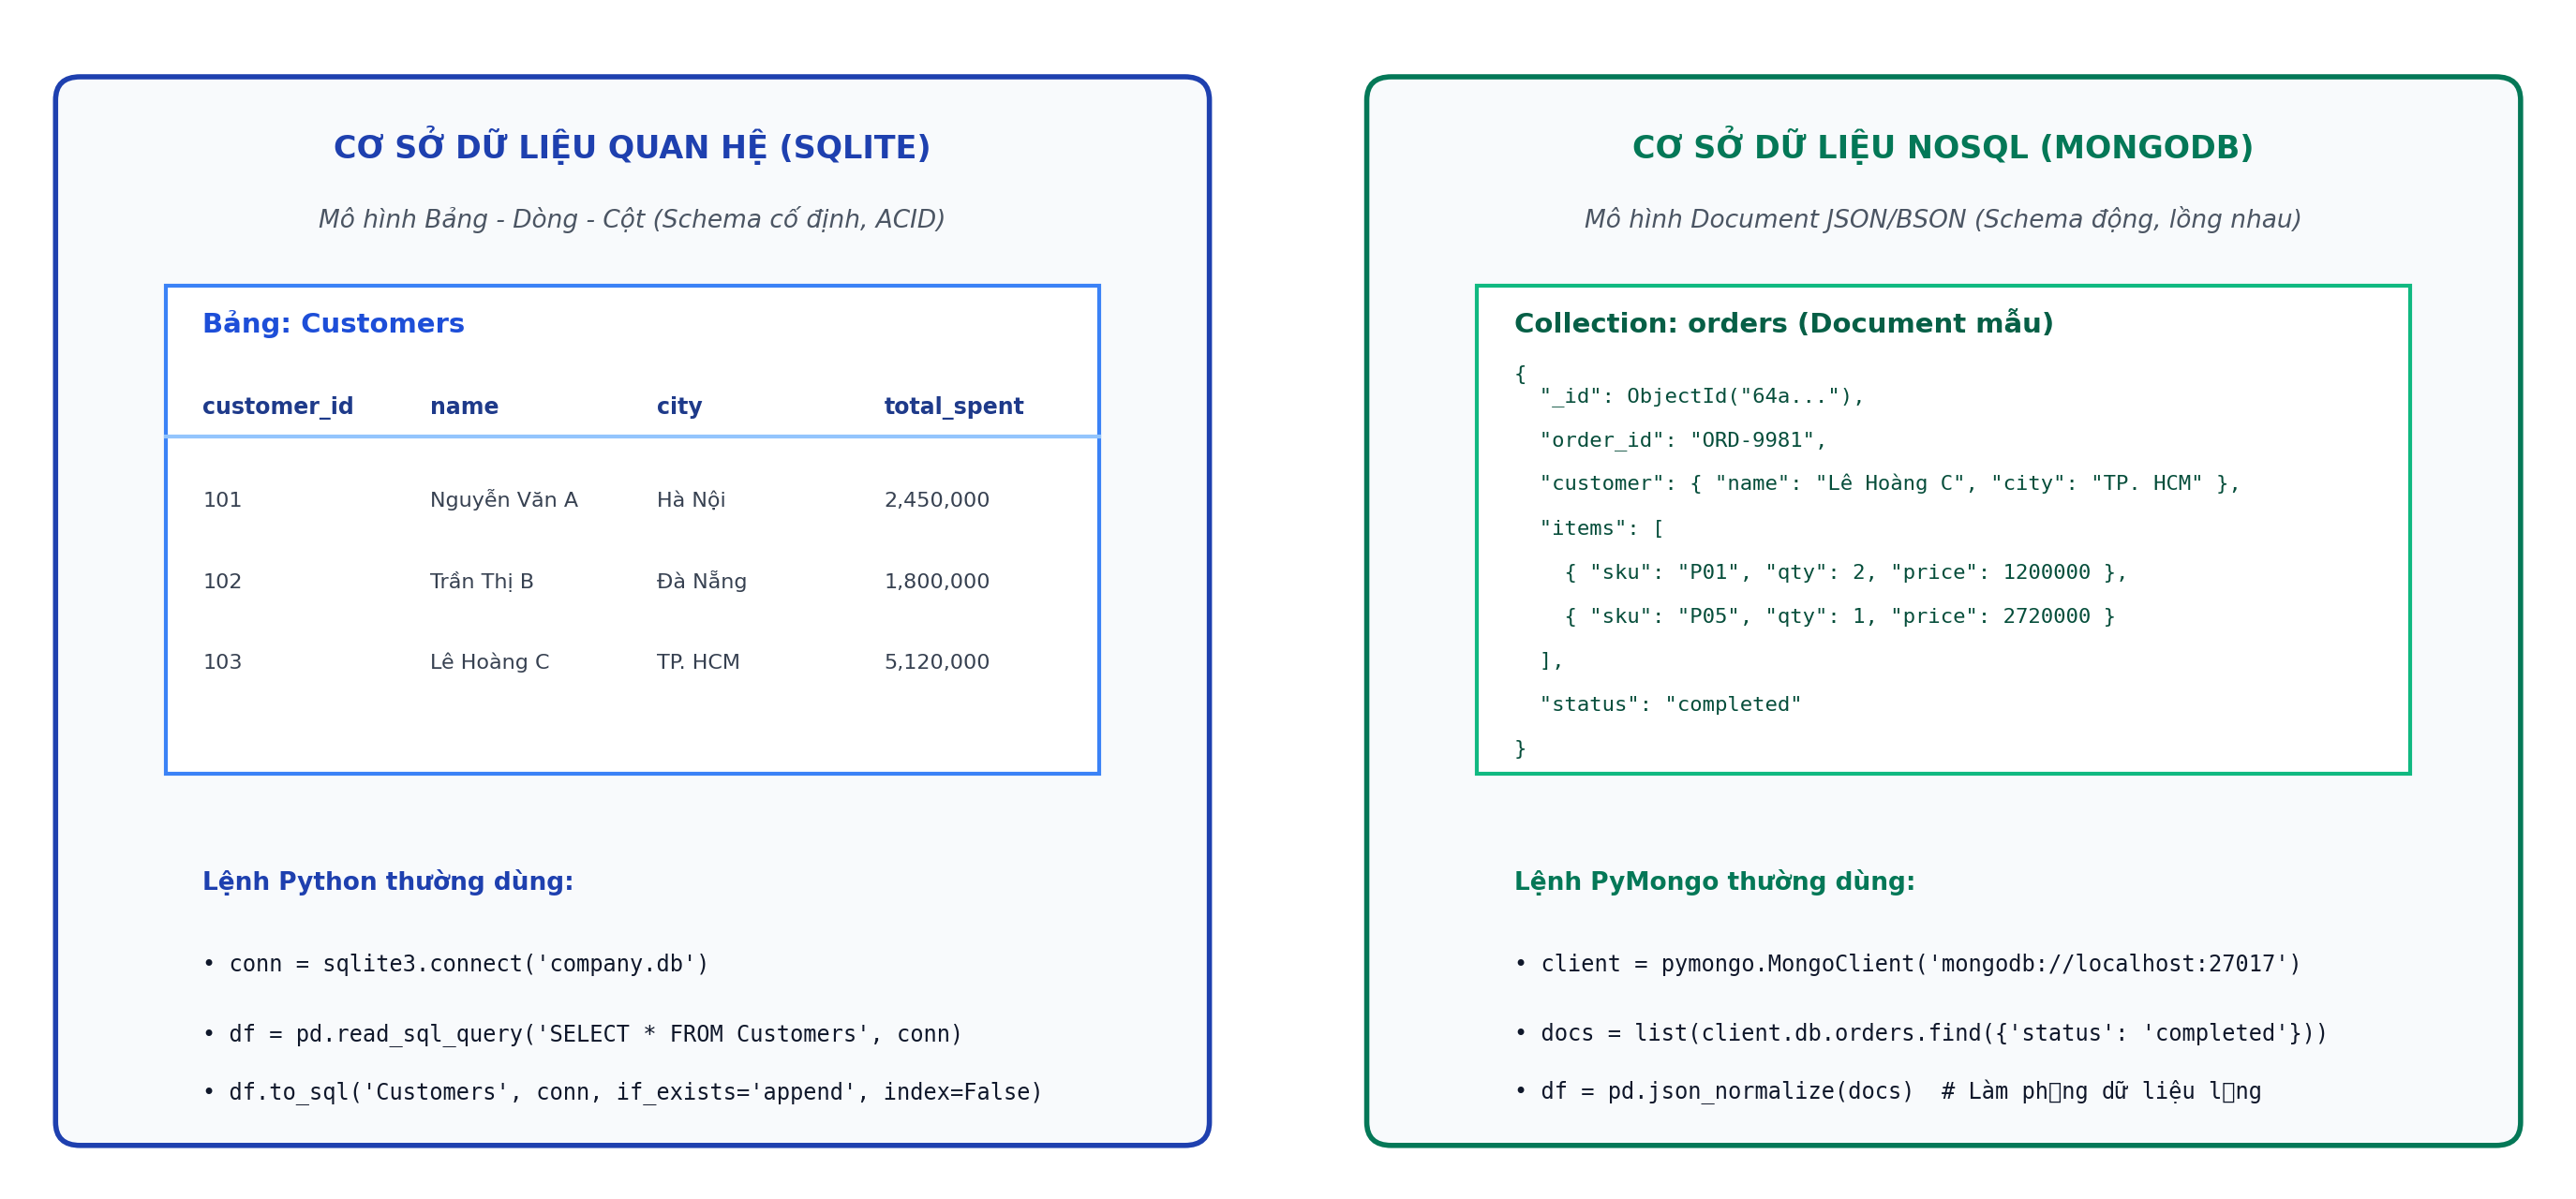
\includegraphics[width=0.92\linewidth]{images/relational-vs-nosql.png}
}{
  \begin{block}{So sánh}
  SQLite: Bảng, Cột, Dòng, ACID, SQL $\longleftrightarrow$ MongoDB: Collections, Documents BSON, Linh hoạt
  \end{block}
}
\end{frame}

\begin{frame}[fragile]{Cơ sở dữ liệu quan hệ SQLite \& Pandas}
\small
\begin{lstlisting}[style=py]
import sqlite3, pandas as pd

conn = sqlite3.connect("data/company.db")

# 1. Truy van JOIN phuc tap truc tiep vao DataFrame
query = (
    "SELECT e.emp_id, e.full_name, d.dept_name, SUM(s.revenue) AS total_revenue "
    "FROM employees e "
    "JOIN departments d ON e.dept_id = d.dept_id "
    "JOIN monthly_sales s ON e.emp_id = s.emp_id "
    "GROUP BY e.emp_id, e.full_name, d.dept_name "
    "ORDER BY total_revenue DESC;"
)
df_sales = pd.read_sql_query(query, conn)

# 2. Luu tru nguoc tro lai co so du lieu SQLite
df_sales.to_sql("top_sales_summary", conn, if_exists="replace", index=False)
conn.close()
\end{lstlisting}
\end{frame}

\begin{frame}[fragile]{Cơ sở dữ liệu NoSQL MongoDB (\cmd{pymongo})}
\small
\begin{lstlisting}[style=py]
from pymongo import MongoClient
import pandas as pd

# Ket noi cluster / local instance
client = MongoClient("mongodb://localhost:27017/")
db = client["retail_store_db"]
orders_col = db["customer_orders"]

# Truong hop 1: Chen document linh hoat
orders_col.insert_one({"order_id": "ORD-101", "items": ["P01", "P02"], "amount": 2500000})

# Truong hop 2: Loc du lieu va chuyen sang Pandas DataFrame
cursor = orders_col.find({"amount": {"$gte": 1000000}})
df_orders = pd.json_normalize(list(cursor))

# Xu ly khoa dac thu BSON ObjectId
if "_id" in df_orders.columns:
    df_orders["_id"] = df_orders["_id"].astype(str)
\end{lstlisting}
\end{frame}

\begin{frame}{Bảng tổng kết tra cứu nhanh I/O trong Data Science}
\small
\begin{table}[]
\centering
\begin{tabular}{llll}
\toprule
\textbf{Định dạng} & \textbf{Hàm Đọc (Read)} & \textbf{Hàm Ghi (Write)} & \textbf{Thư viện chính} \\
\midrule
CSV / TSV & \cmd{pd.read_csv()} & \cmd{df.to_csv()} & Pandas (built-in) \\
Excel & \cmd{pd.read_excel()} & \cmd{df.to_excel()} & \cmd{openpyxl} \\
JSON & \cmd{pd.json_normalize()} & \cmd{df.to_json()} & \cmd{json}, Pandas \\
HTML & \cmd{pd.read_html()} & \cmd{df.to_html()} & \cmd{lxml}, \cmd{bs4} \\
PDF & \cmd{page.extract_tables()} & -- & \cmd{pdfplumber} \\
SQLite & \cmd{pd.read_sql_query()} & \cmd{df.to_sql()} & \cmd{sqlite3}, SQLAlchemy \\
MongoDB & \cmd{col.find() -> DF} & \cmd{col.insert_many()} & \cmd{pymongo} \\
\bottomrule
\end{tabular}
\end{table}
\begin{alertblock}{Nguyên tắc vàng về An toàn \& Hiệu năng}
1. Luôn dùng tham số hóa (\cmd{?}) chống SQL Injection.  
2. Quản lý tài nguyên qua ngữ cảnh \cmd{with}.  
3. Sử dụng \cmd{usecols} và \cmd{chunksize} khi làm việc với tập dữ liệu quy mô lớn.
\end{alertblock}
\end{frame}

\begin{frame}{Tổng kết \& Câu hỏi Thảo luận}
\centering
\vspace{1em}
\key{\Large Chúc các bạn thực hành hiệu quả!}
\vspace{1em}

\begin{block}{Câu hỏi suy ngẫm cho buổi thực hành}
\begin{enumerate}
  \item Khi nào nên lưu trữ đơn hàng dưới dạng NoSQL Document thay vì bảng cơ sở dữ liệu quan hệ?
  \item Làm thế nào để tự động hóa đường ống tải dữ liệu từ Web API (JSON) vào database SQLite chạy định kỳ mỗi đêm?
\end{enumerate}
\end{block}
\vspace{1em}
\small Liên hệ hỗ trợ: TS. Vũ Đức Minh (\texttt{minhvd@neu.edu.vn})
\end{frame}

\end{document}
